\documentclass[tikz,border=5pt]{standalone}
\usepackage[utf8]{inputenc}
\usepackage[T1]{fontenc}
\usepackage{lmodern,amsmath,amssymb}
\usepackage[american]{circuitikz}
\usepackage{pgfplots}
\pgfplotsset{compat=1.18}
\usetikzlibrary{circuits.logic.US,positioning,calc,arrows.meta,patterns,shapes.geometric}
\definecolor{Primary}{HTML}{1F77B4}
\begin{document}
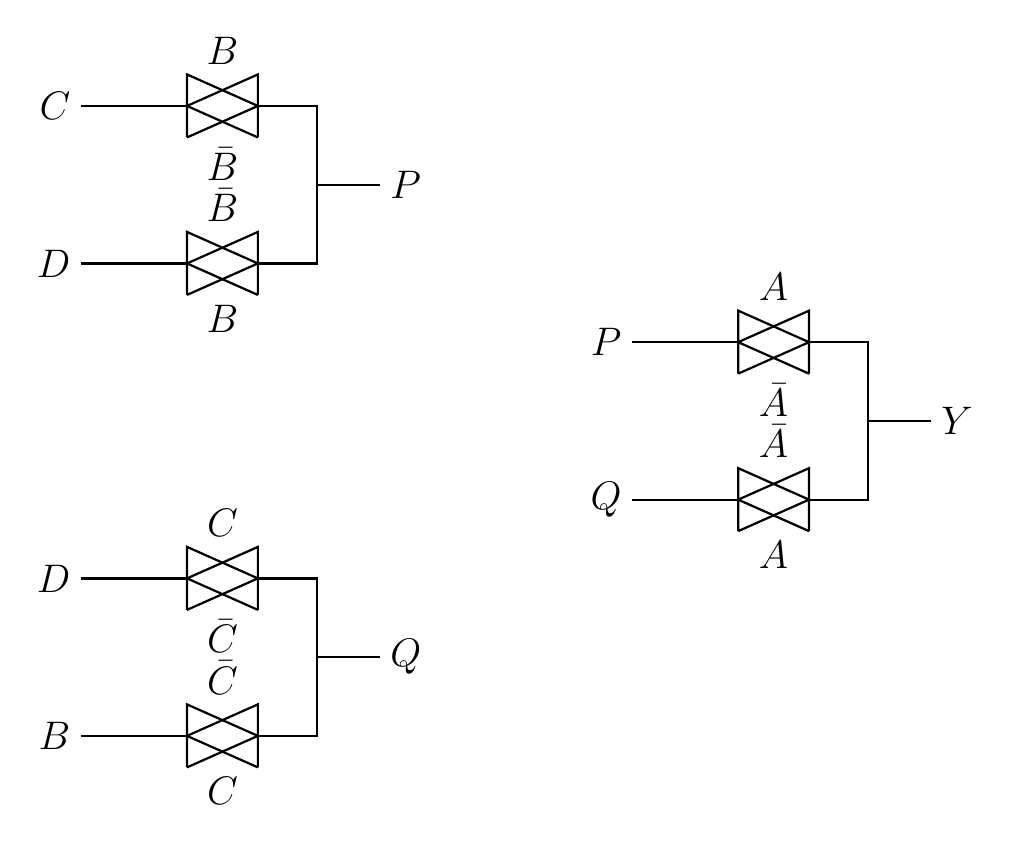
\begin{tikzpicture}[thick,font=\Large]\draw(-0.45,3.6)--(0.45,4)--(-0.45,4.4)--(-0.45,3.6);\draw(0.45,3.6)--(-0.45,4)--(0.45,4.4)--(0.45,3.6);\node[above]at(0,4.4){$ B $};\node[below]at(0,3.6){$ \bar B $};\draw(-0.45,1.6)--(0.45,2)--(-0.45,2.4)--(-0.45,1.6);\draw(0.45,1.6)--(-0.45,2)--(0.45,2.4)--(0.45,1.6);\node[above]at(0,2.4){$ \bar B $};\node[below]at(0,1.6){$ B $};\draw(-1.8,4)node[left]{$ C $}--(-0.45,4);\draw(-1.8,2)node[left]{$ D $}--(-0.45,2);\draw(0.45,4)--(1.2,4)--(1.2,2)--(0.45,2);\draw(1.2,3)--(2,3)node[right]{$ P $};\draw(-0.45,-2.4)--(0.45,-2)--(-0.45,-1.6)--(-0.45,-2.4);\draw(0.45,-2.4)--(-0.45,-2)--(0.45,-1.6)--(0.45,-2.4);\node[above]at(0,-1.6){$ C $};\node[below]at(0,-2.4){$ \bar C $};\draw(-0.45,-4.4)--(0.45,-4)--(-0.45,-3.6)--(-0.45,-4.4);\draw(0.45,-4.4)--(-0.45,-4)--(0.45,-3.6)--(0.45,-4.4);\node[above]at(0,-3.6){$ \bar C $};\node[below]at(0,-4.4){$ C $};\draw(-1.8,-2)node[left]{$ D $}--(-0.45,-2);\draw(-1.8,-4)node[left]{$ B $}--(-0.45,-4);\draw(0.45,-2)--(1.2,-2)--(1.2,-4)--(0.45,-4);\draw(1.2,-3)--(2,-3)node[right]{$ Q $};\draw(6.55,0.6)--(7.45,1)--(6.55,1.4)--(6.55,0.6);\draw(7.45,0.6)--(6.55,1)--(7.45,1.4)--(7.45,0.6);\node[above]at(7,1.4){$ A $};\node[below]at(7,0.6){$ \bar A $};\draw(6.55,-1.4)--(7.45,-1)--(6.55,-0.6)--(6.55,-1.4);\draw(7.45,-1.4)--(6.55,-1)--(7.45,-0.6)--(7.45,-1.4);\node[above]at(7,-0.6){$ \bar A $};\node[below]at(7,-1.4){$ A $};\draw(5.2,1)node[left]{$ P $}--(6.55,1);\draw(5.2,-1)node[left]{$ Q $}--(6.55,-1);\draw(7.45,1)--(8.2,1)--(8.2,-1)--(7.45,-1);\draw(8.2,0)--(9,0)node[right]{$ Y $};\end{tikzpicture}
\end{document}
